\begin{figure}
    \centering
    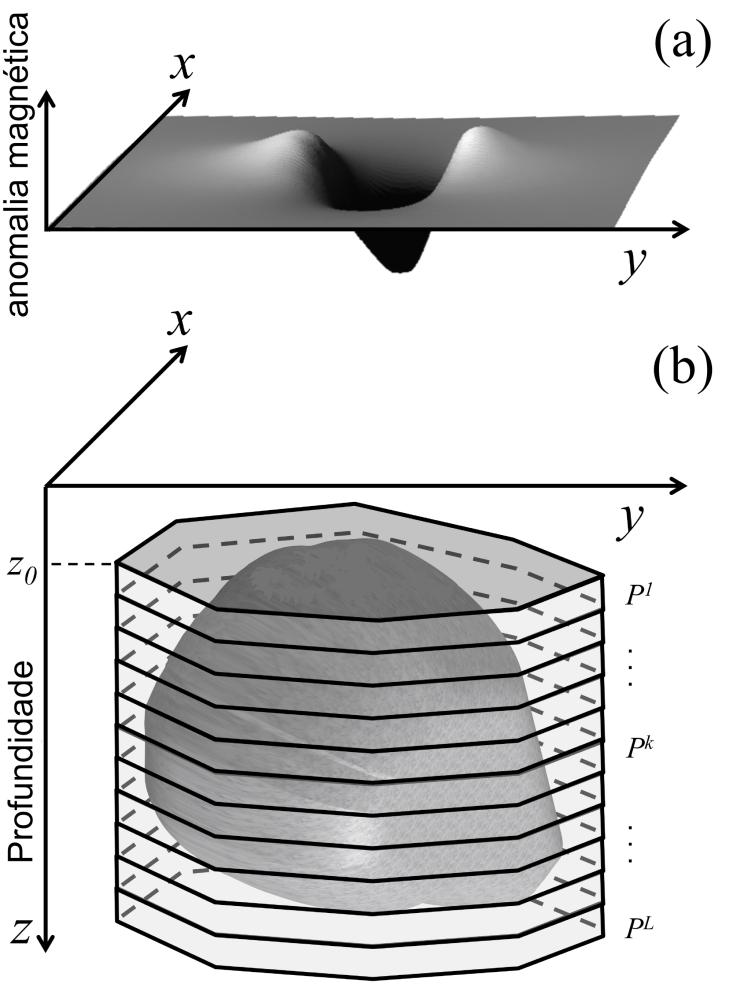
\includegraphics[scale=0.3]{figures/observed_data.png}
    \caption{Schematic representation of (a) total-filed anomaly (gray surface) produced by (b) a 3-D anomalous source (dark gray volume). The interpretation model in (b) consists of a set of L vertical, juxtaposed 3-D prisms $P^k$ , $k = 1,\dots, L$, (light gray prisms) in the vertical direction of a right-handed coordinate system.}
    \label{fig:obs}
\end{figure}

\begin{figure}
    \centering
    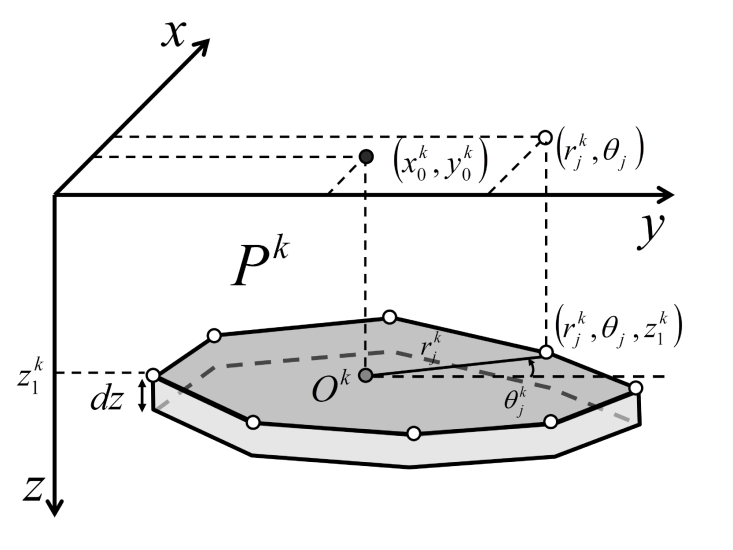
\includegraphics[scale=0.3]{figures/prism_parameters_mod.png}
    \caption{Polygonal cross-section of the $k$th vertical prism $P^k$ described by $V$ vertices (white dots) with polar coordinates ($r^k_j$ , $\theta ^k_j$), $j = 1, \dots, V$, $k = 1, \dots, L$ , referred to an arbitrary origin $O^k$ (grey dot) with horizontal Cartesian coordinates ($x_0^k$ , $y_0^k$), $k = 1, \dots, L$ , (black dot).}
    \label{fig:prism_parameters}
\end{figure}

\begin{figure}
    \centering
    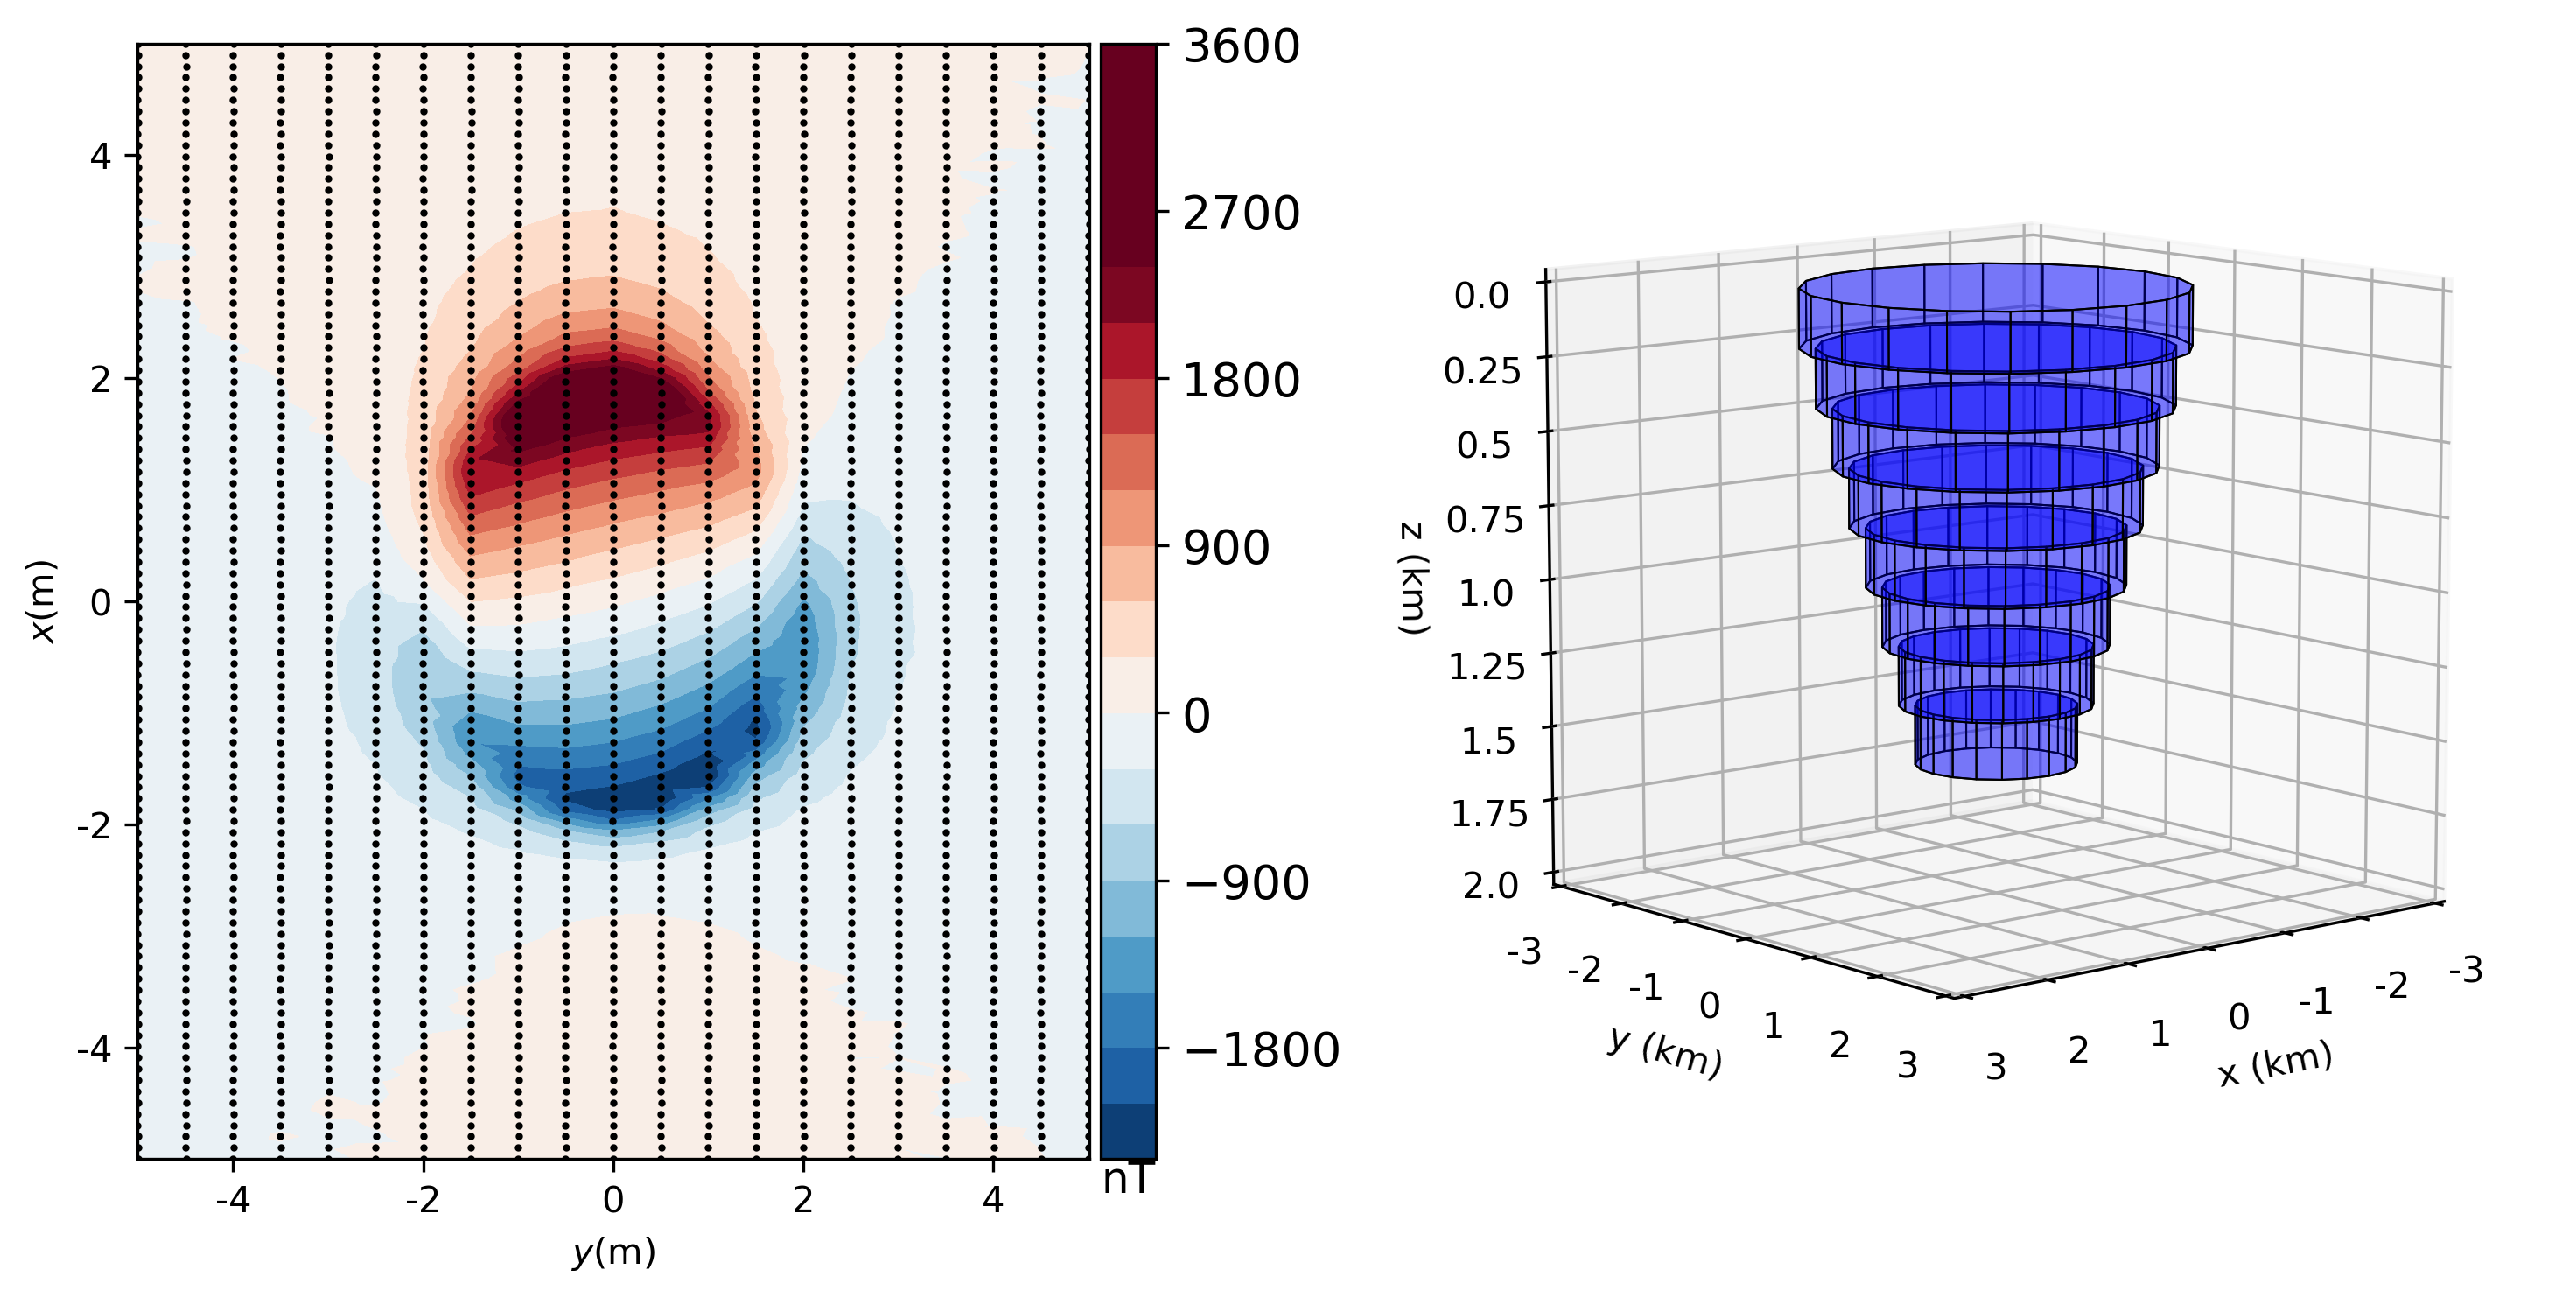
\includegraphics[scale=.5]{figures/wedding_cake_model_data.png}
    \caption{Simple model simulation. (a) noise-corrupted total-field anomaly produced by the simple model (blue prisms) in (b). The black dots represent the observation points simulating an airborne survey.
}
    \label{fig:kimb_model}
\end{figure}

\begin{figure}
	\centering
	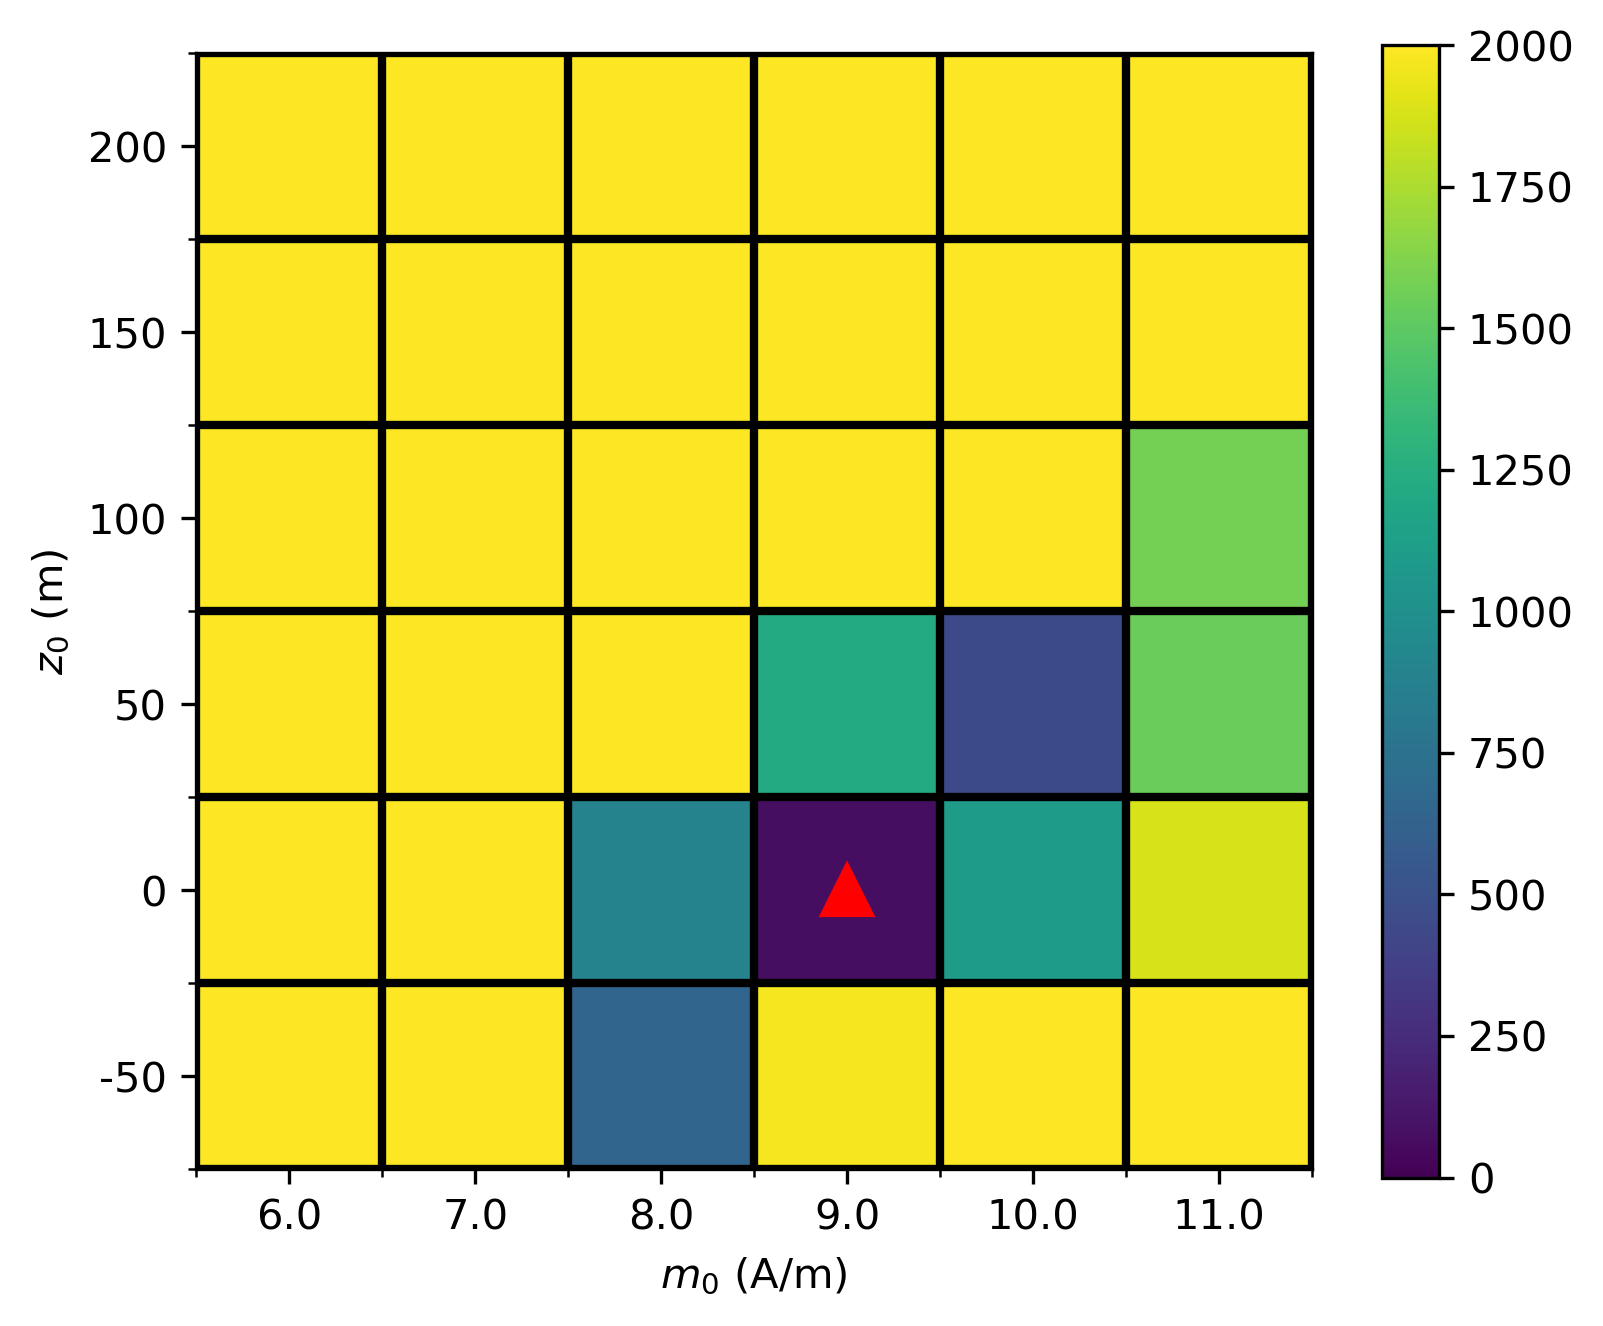
\includegraphics[scale=.75]{figures/wedding_cake_obj_func_map.png}
	\caption{Map of the objective function values due to the inverse solutions for the simple model. The range of $m_0$ varies from $6$ to $11$ A/m in a step of $1$ A/m and the range of $z_0$ varies from $-50$ to $200$ m in a step of $50$ m. Each square is a value of the goal function (eq. \ref{eq:gamma}) of a solution of the inverse problem for a pair of the total-magnetization intensity and the depth to the top of the source. The red triangle represents the true values for $m_0 = 9$ A/m and $z_0=0$m.
	}
	\label{fig:kimb_map}
\end{figure}

\begin{figure}
	\centering
	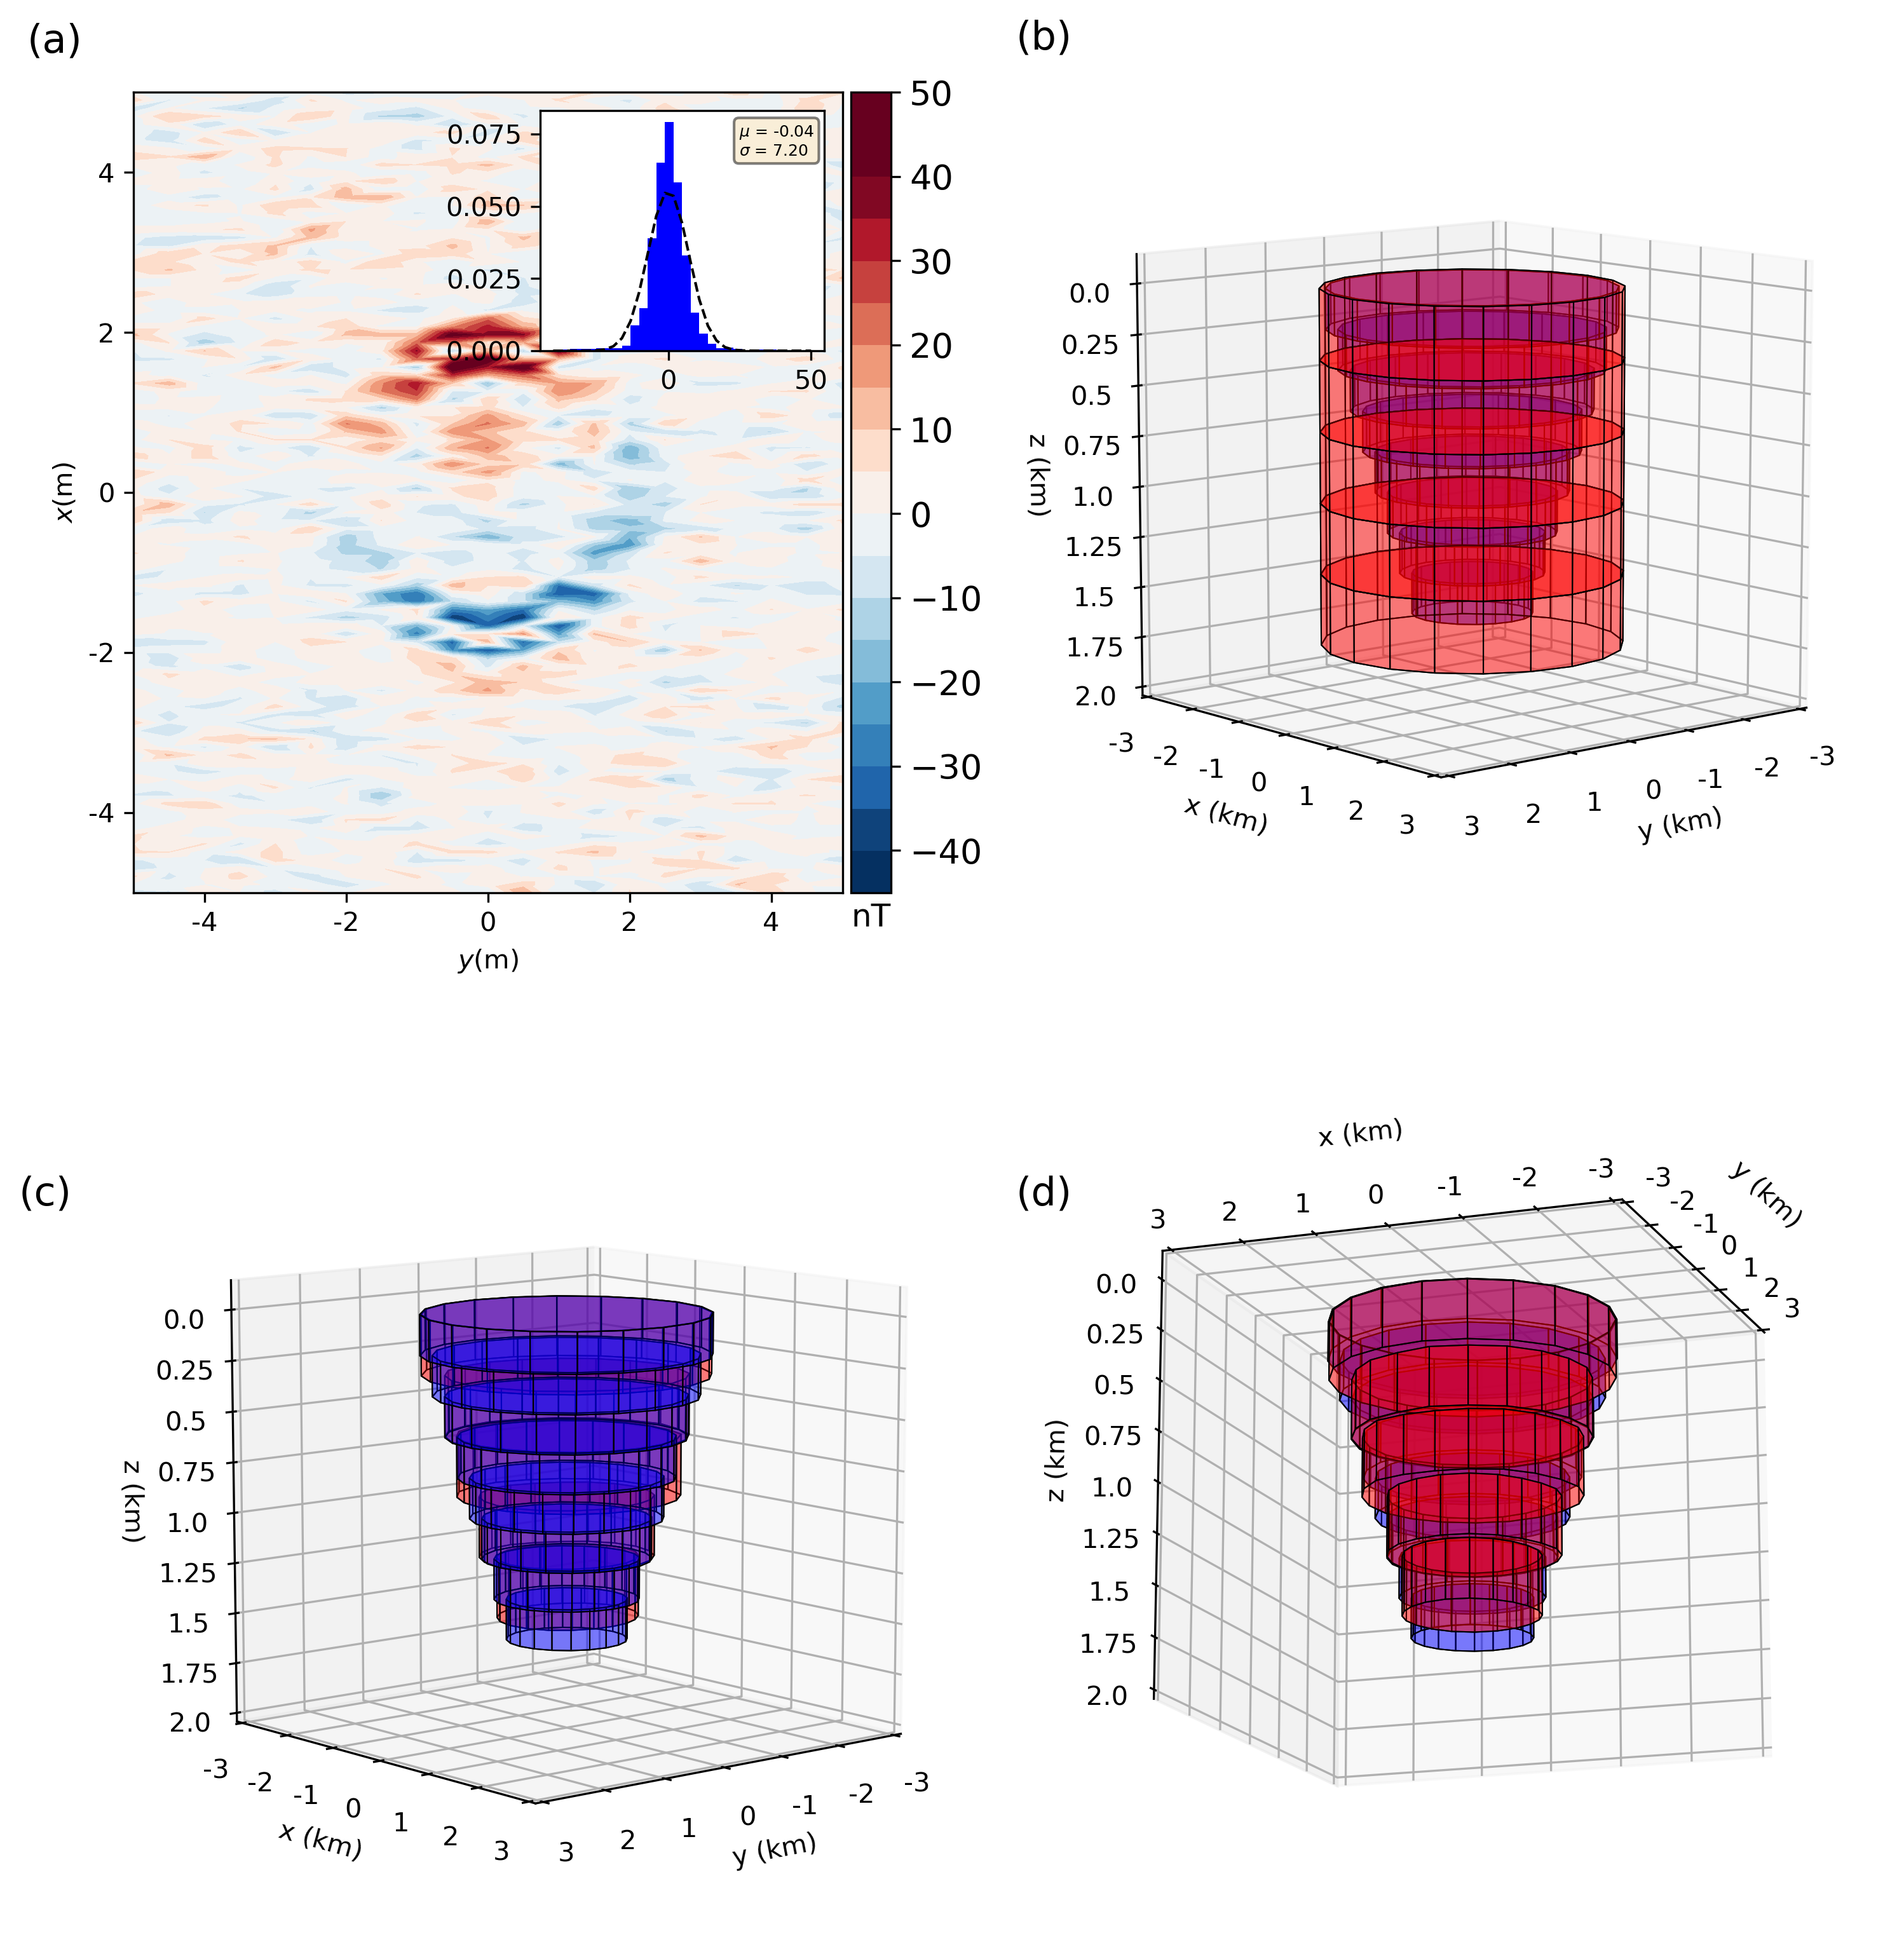
\includegraphics[scale=.5]{figures/wedding_cake_results.png}
	\caption{Application to simple model data. (a) residual data given by the difference between the noise-corrupted data (Fig. \ref{fig:kimb_model}(a)) and the predicted data (not shown) produced by the inverse model (red prisms) in (c) and (d). These inversions were computed using the same cylinder as a initial approximation. The red prisms in (b) represent the input model of the inversion.
	}
	\label{fig:kimb_results}
\end{figure}

\begin{figure}
    \centering
    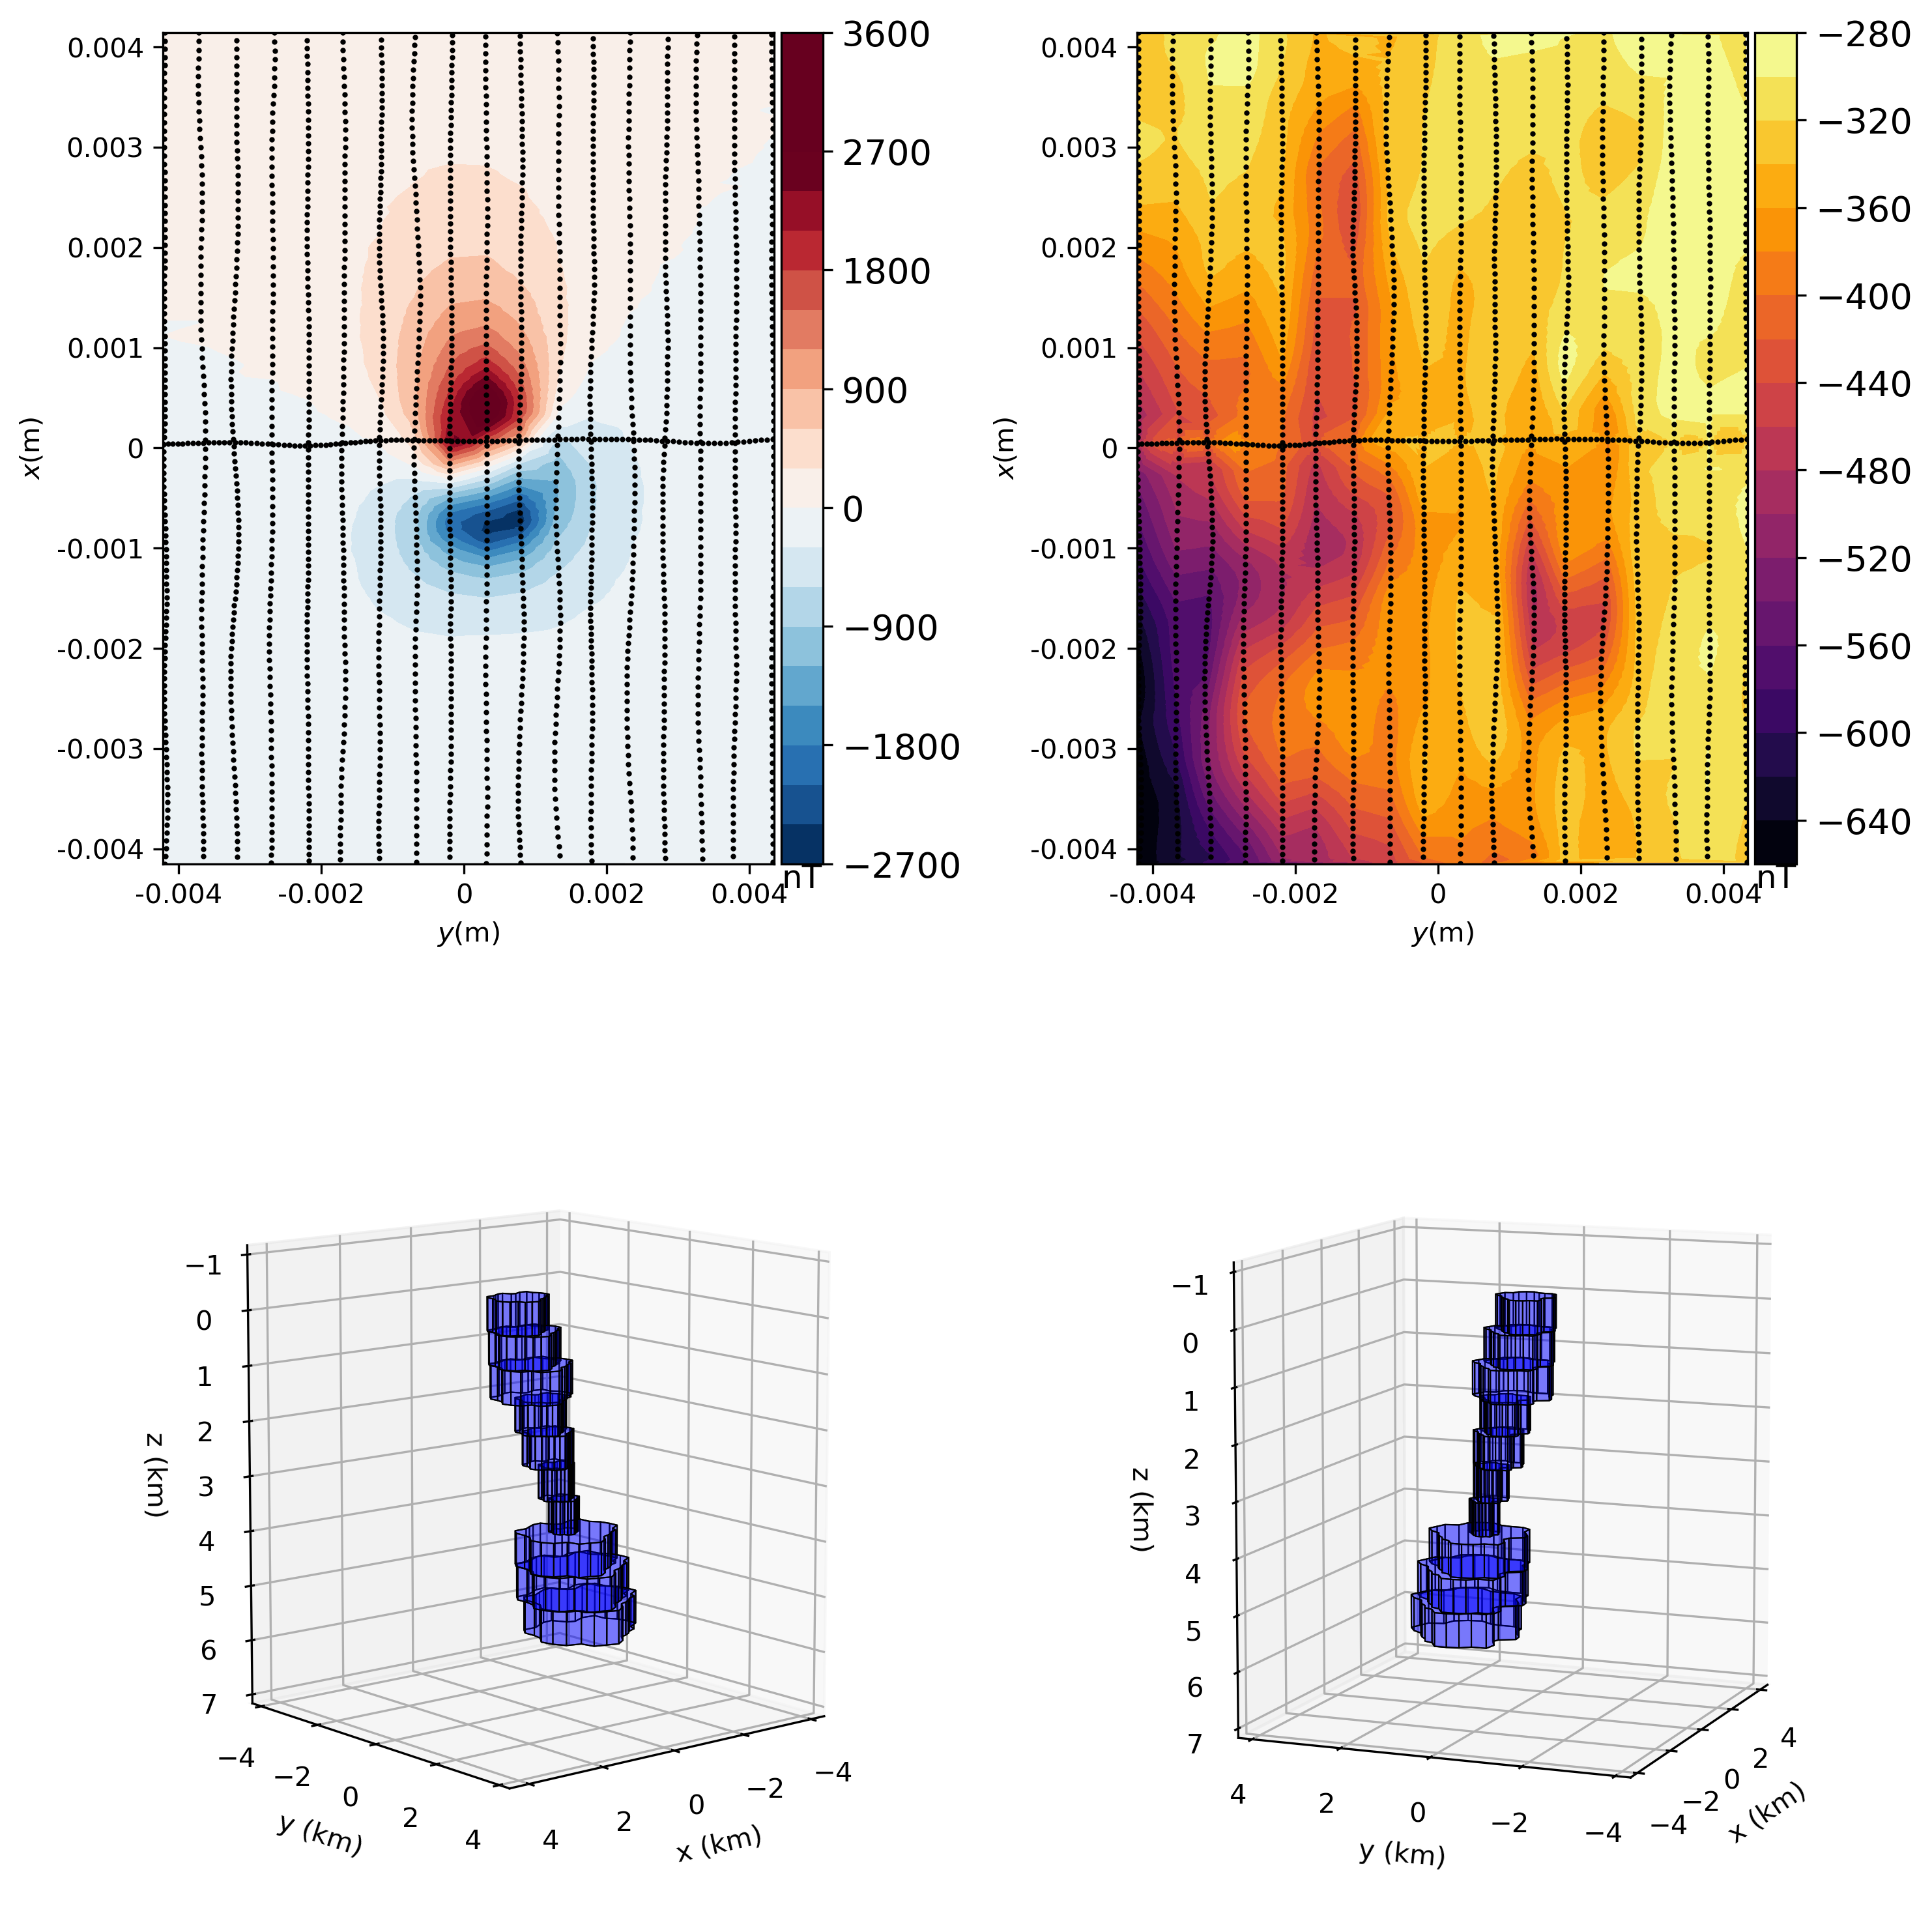
\includegraphics[scale=.5]{figures/complex_model_data.png}
    \caption{Complex model simulation. (a) noise-corrupted total-field anomaly produced by the complex model (blue prisms) in (c) and (d). The black dots represent the observation points that simulate an airborne survey.
}
    \label{fig:complex_model}
\end{figure}

\begin{figure}
	\centering
	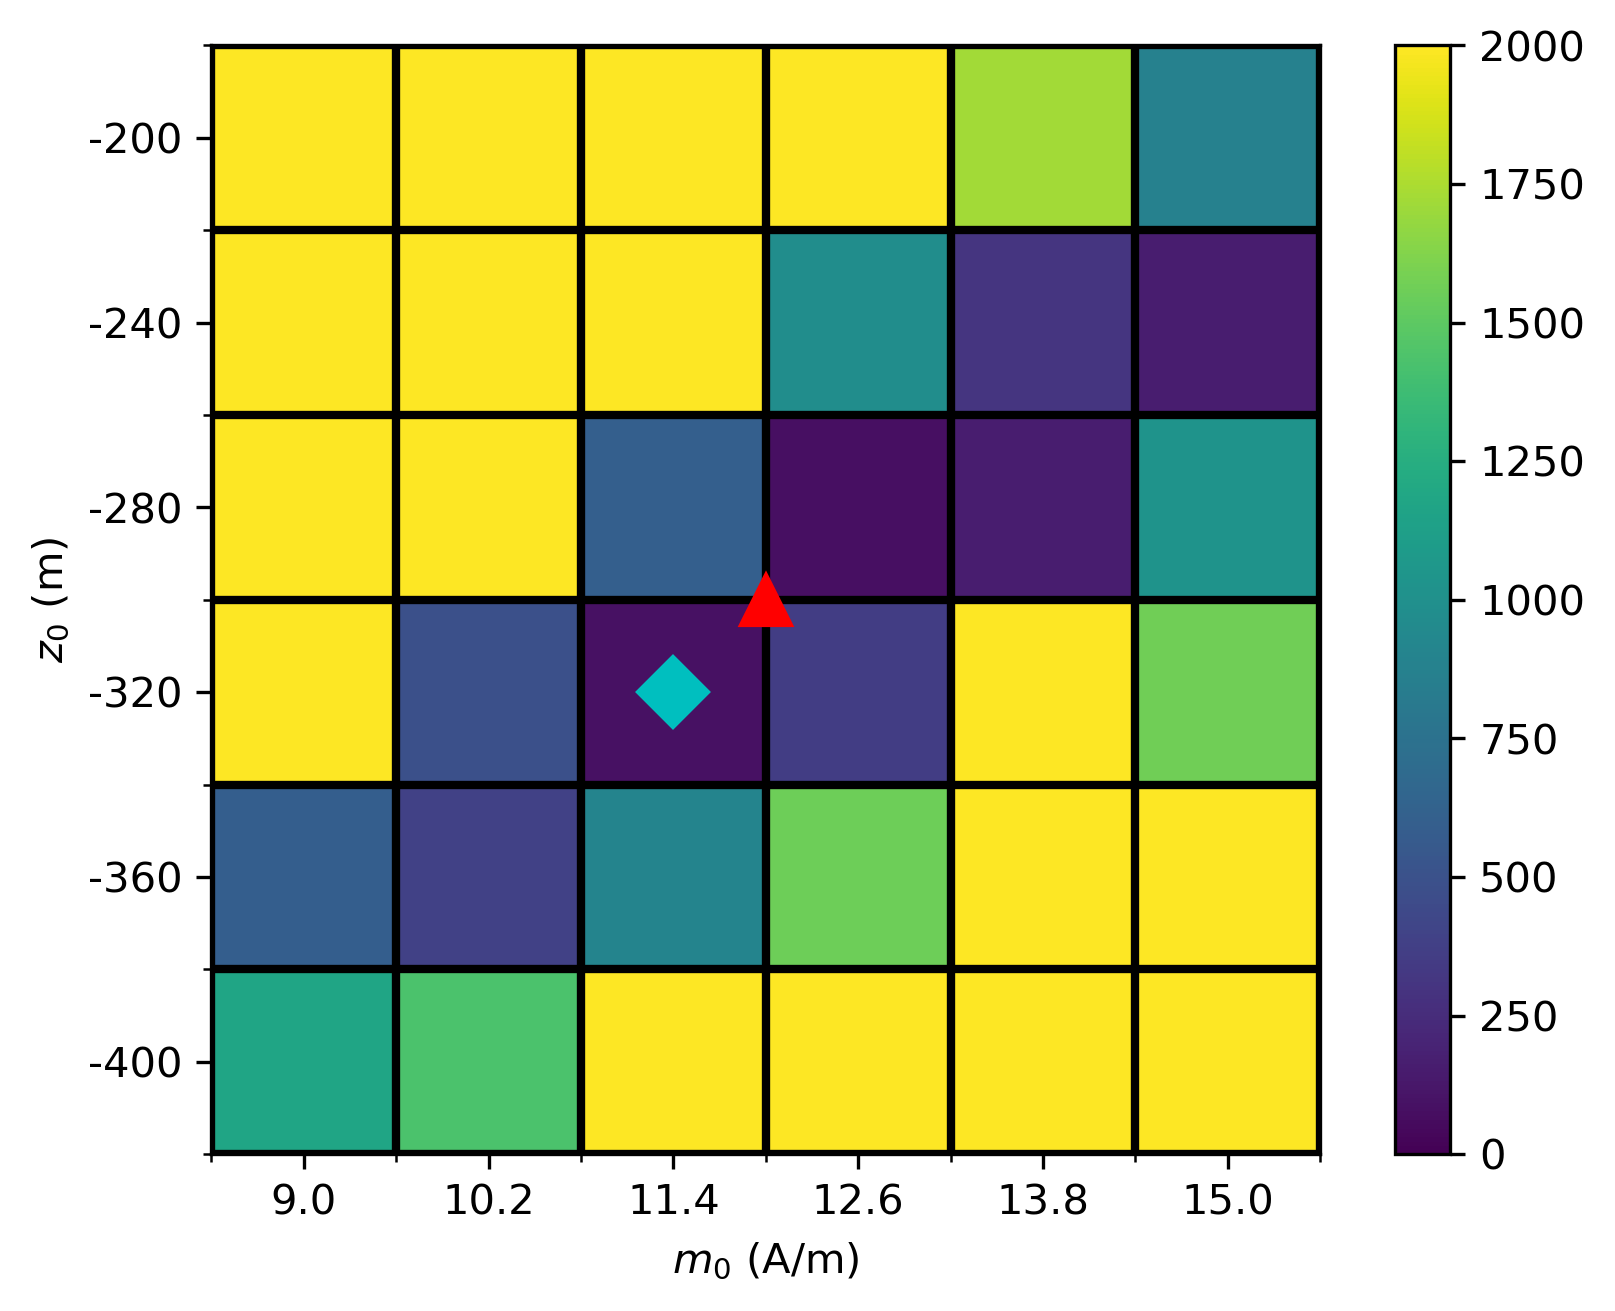
\includegraphics[scale=.75]{figures/complex_obj_func_map.png}
	\caption{Map of the objective function values due to the inverse solutions for the complex model. The range of $m_0$ varies from $9$ to $15$ A/m in a step of $1.2$ A/m and the range of $z_0$ varies from $-400$ to $-200$ m in a step of $50$ m. Each square is a value of the goal function (eq. \ref{eq:gamma}) of a solution of the inverse problem for a pair of the total-magnetization intensity and the depth to the top of the source. These inversions were computed using the same cylinder as a initial approximation. The red triangle represents the true values for $m_0$ and $z_0$. The cyan diamond represents the solution with the lowest function value.
	}
	\label{fig:complex_map}
\end{figure}

\begin{figure}
    \centering
    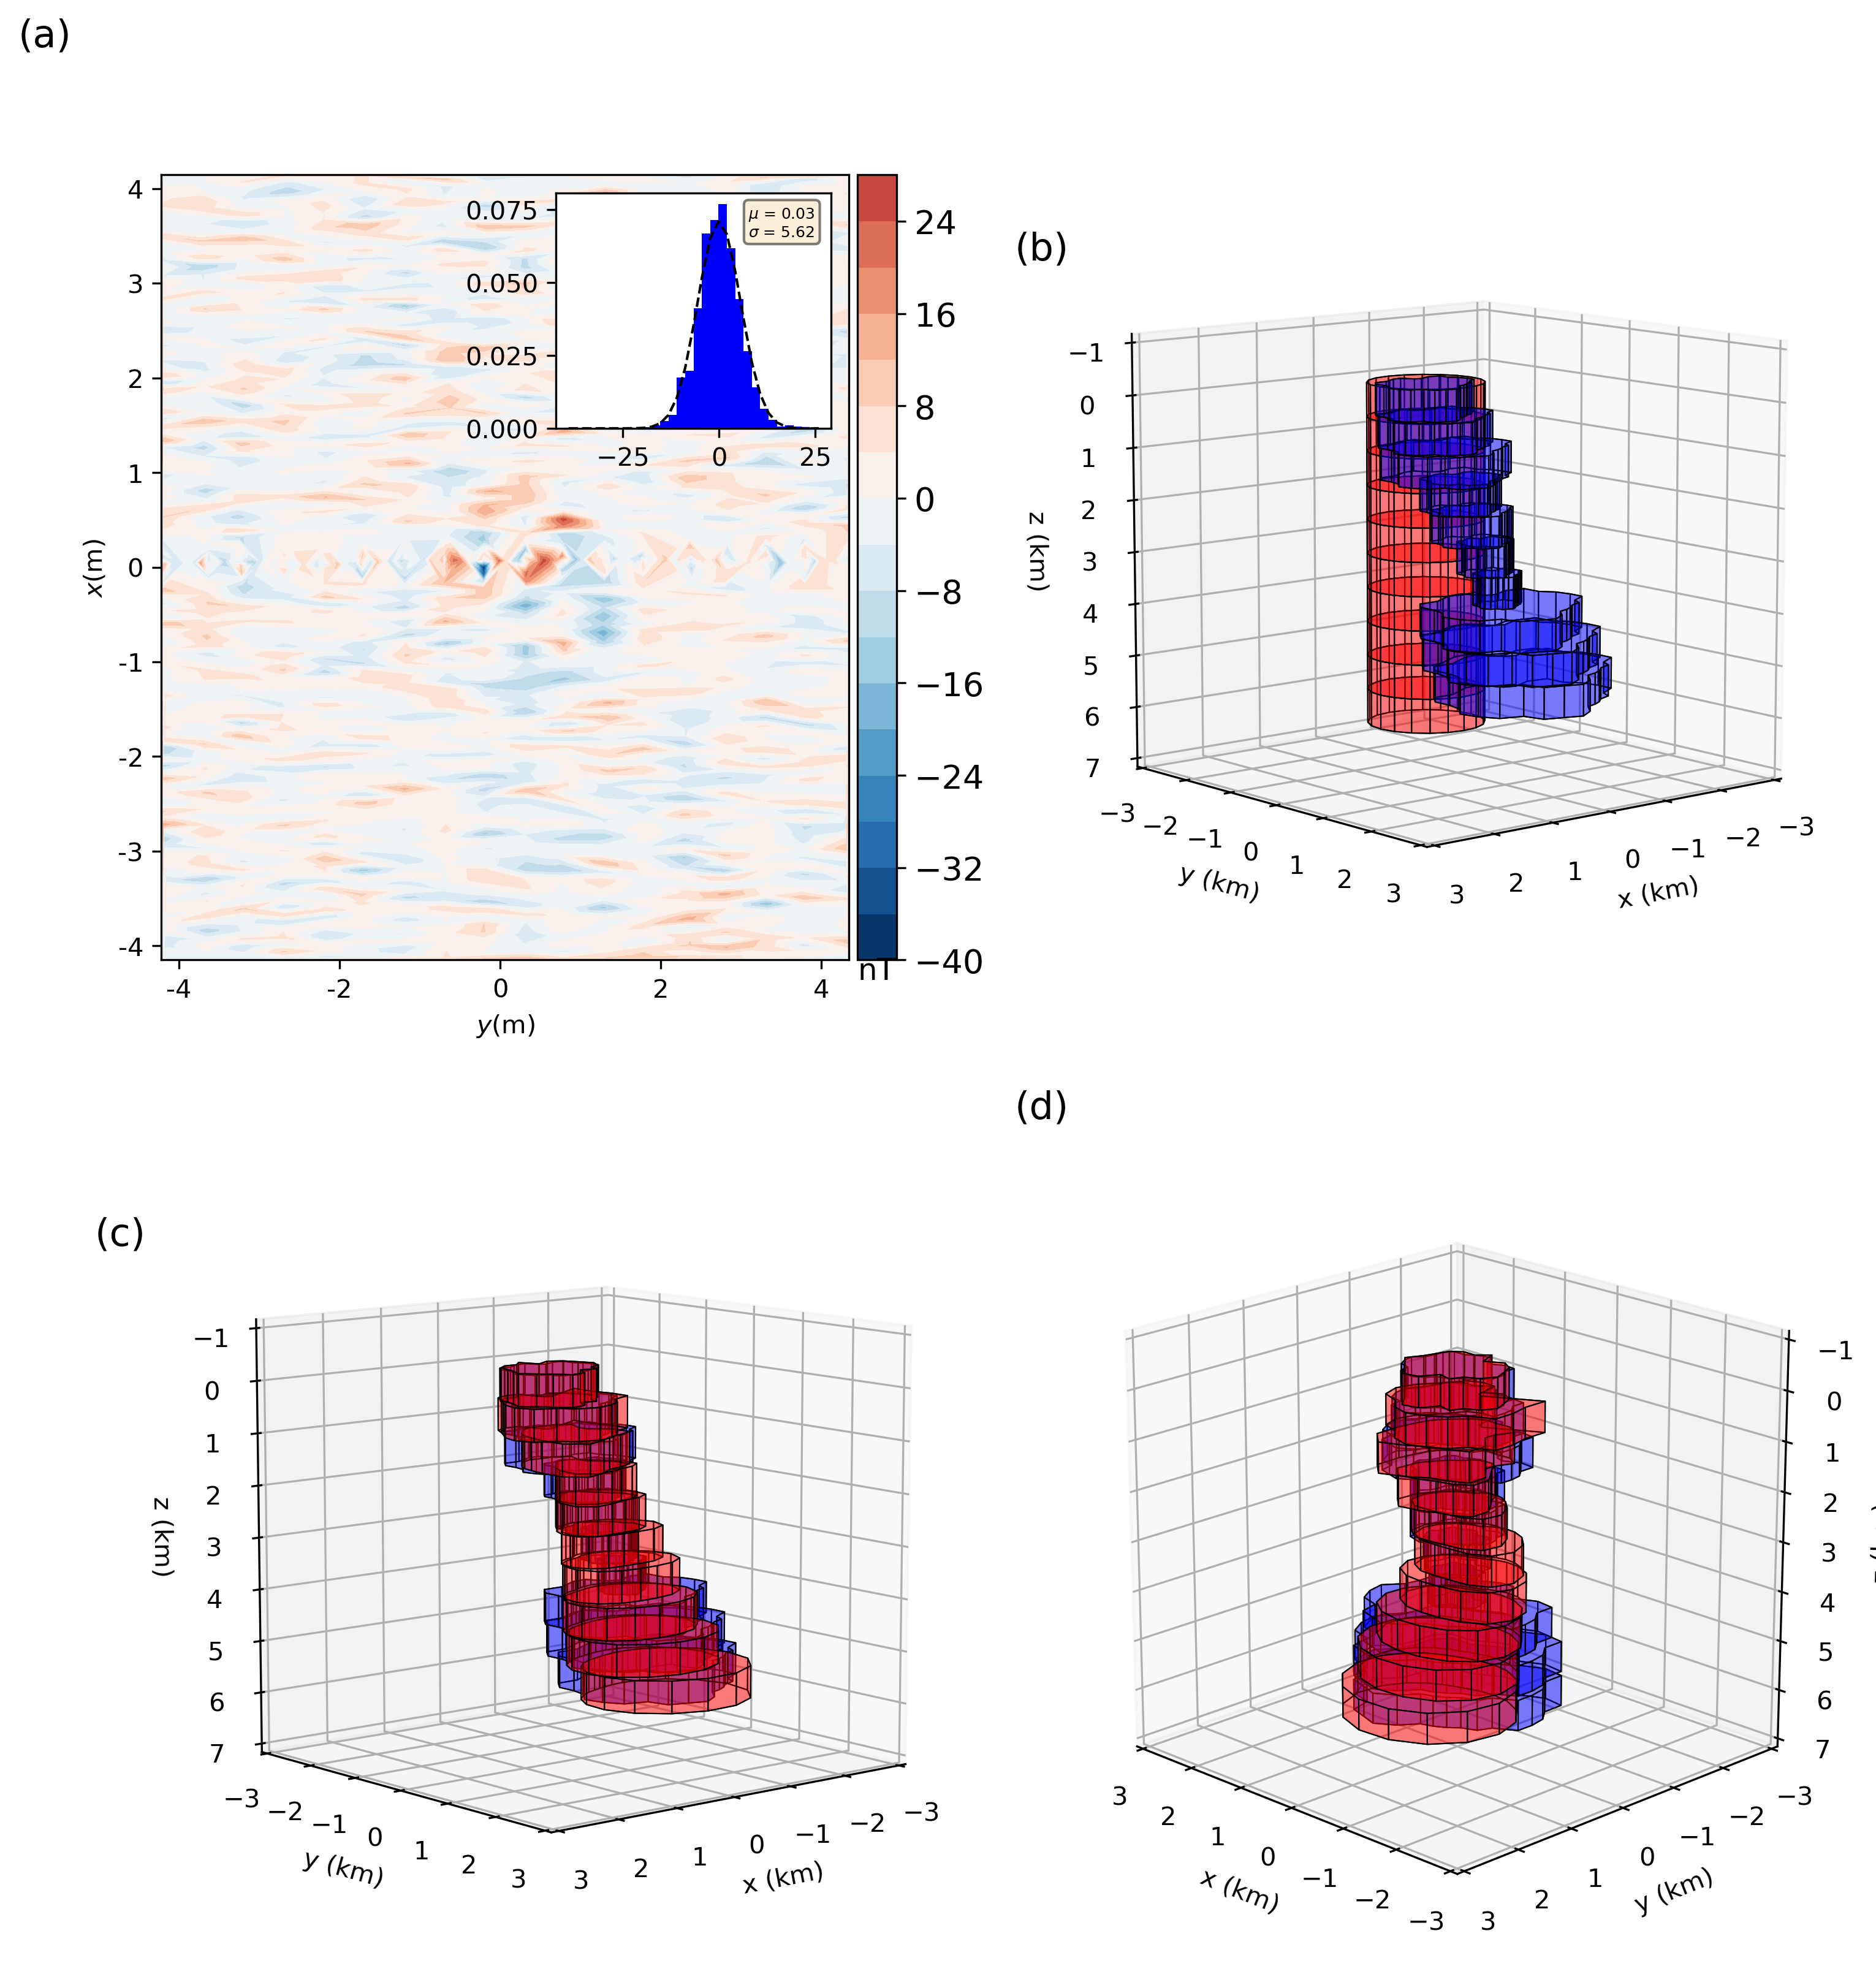
\includegraphics[scale=.5]{figures/complex_results.png}
    \caption{Application to complex model data. (a) residual data given by the difference between the noise-corrupted data (Fig. \ref{fig:complex_model}(a)) and the predicted data (not shown) produced by the inverse model (red prisms) in (c) and (d). The red prisms in (b) represent the input model of the inversion.
}
    \label{fig:complex_result}
\end{figure}

\begin{figure}
    \centering
    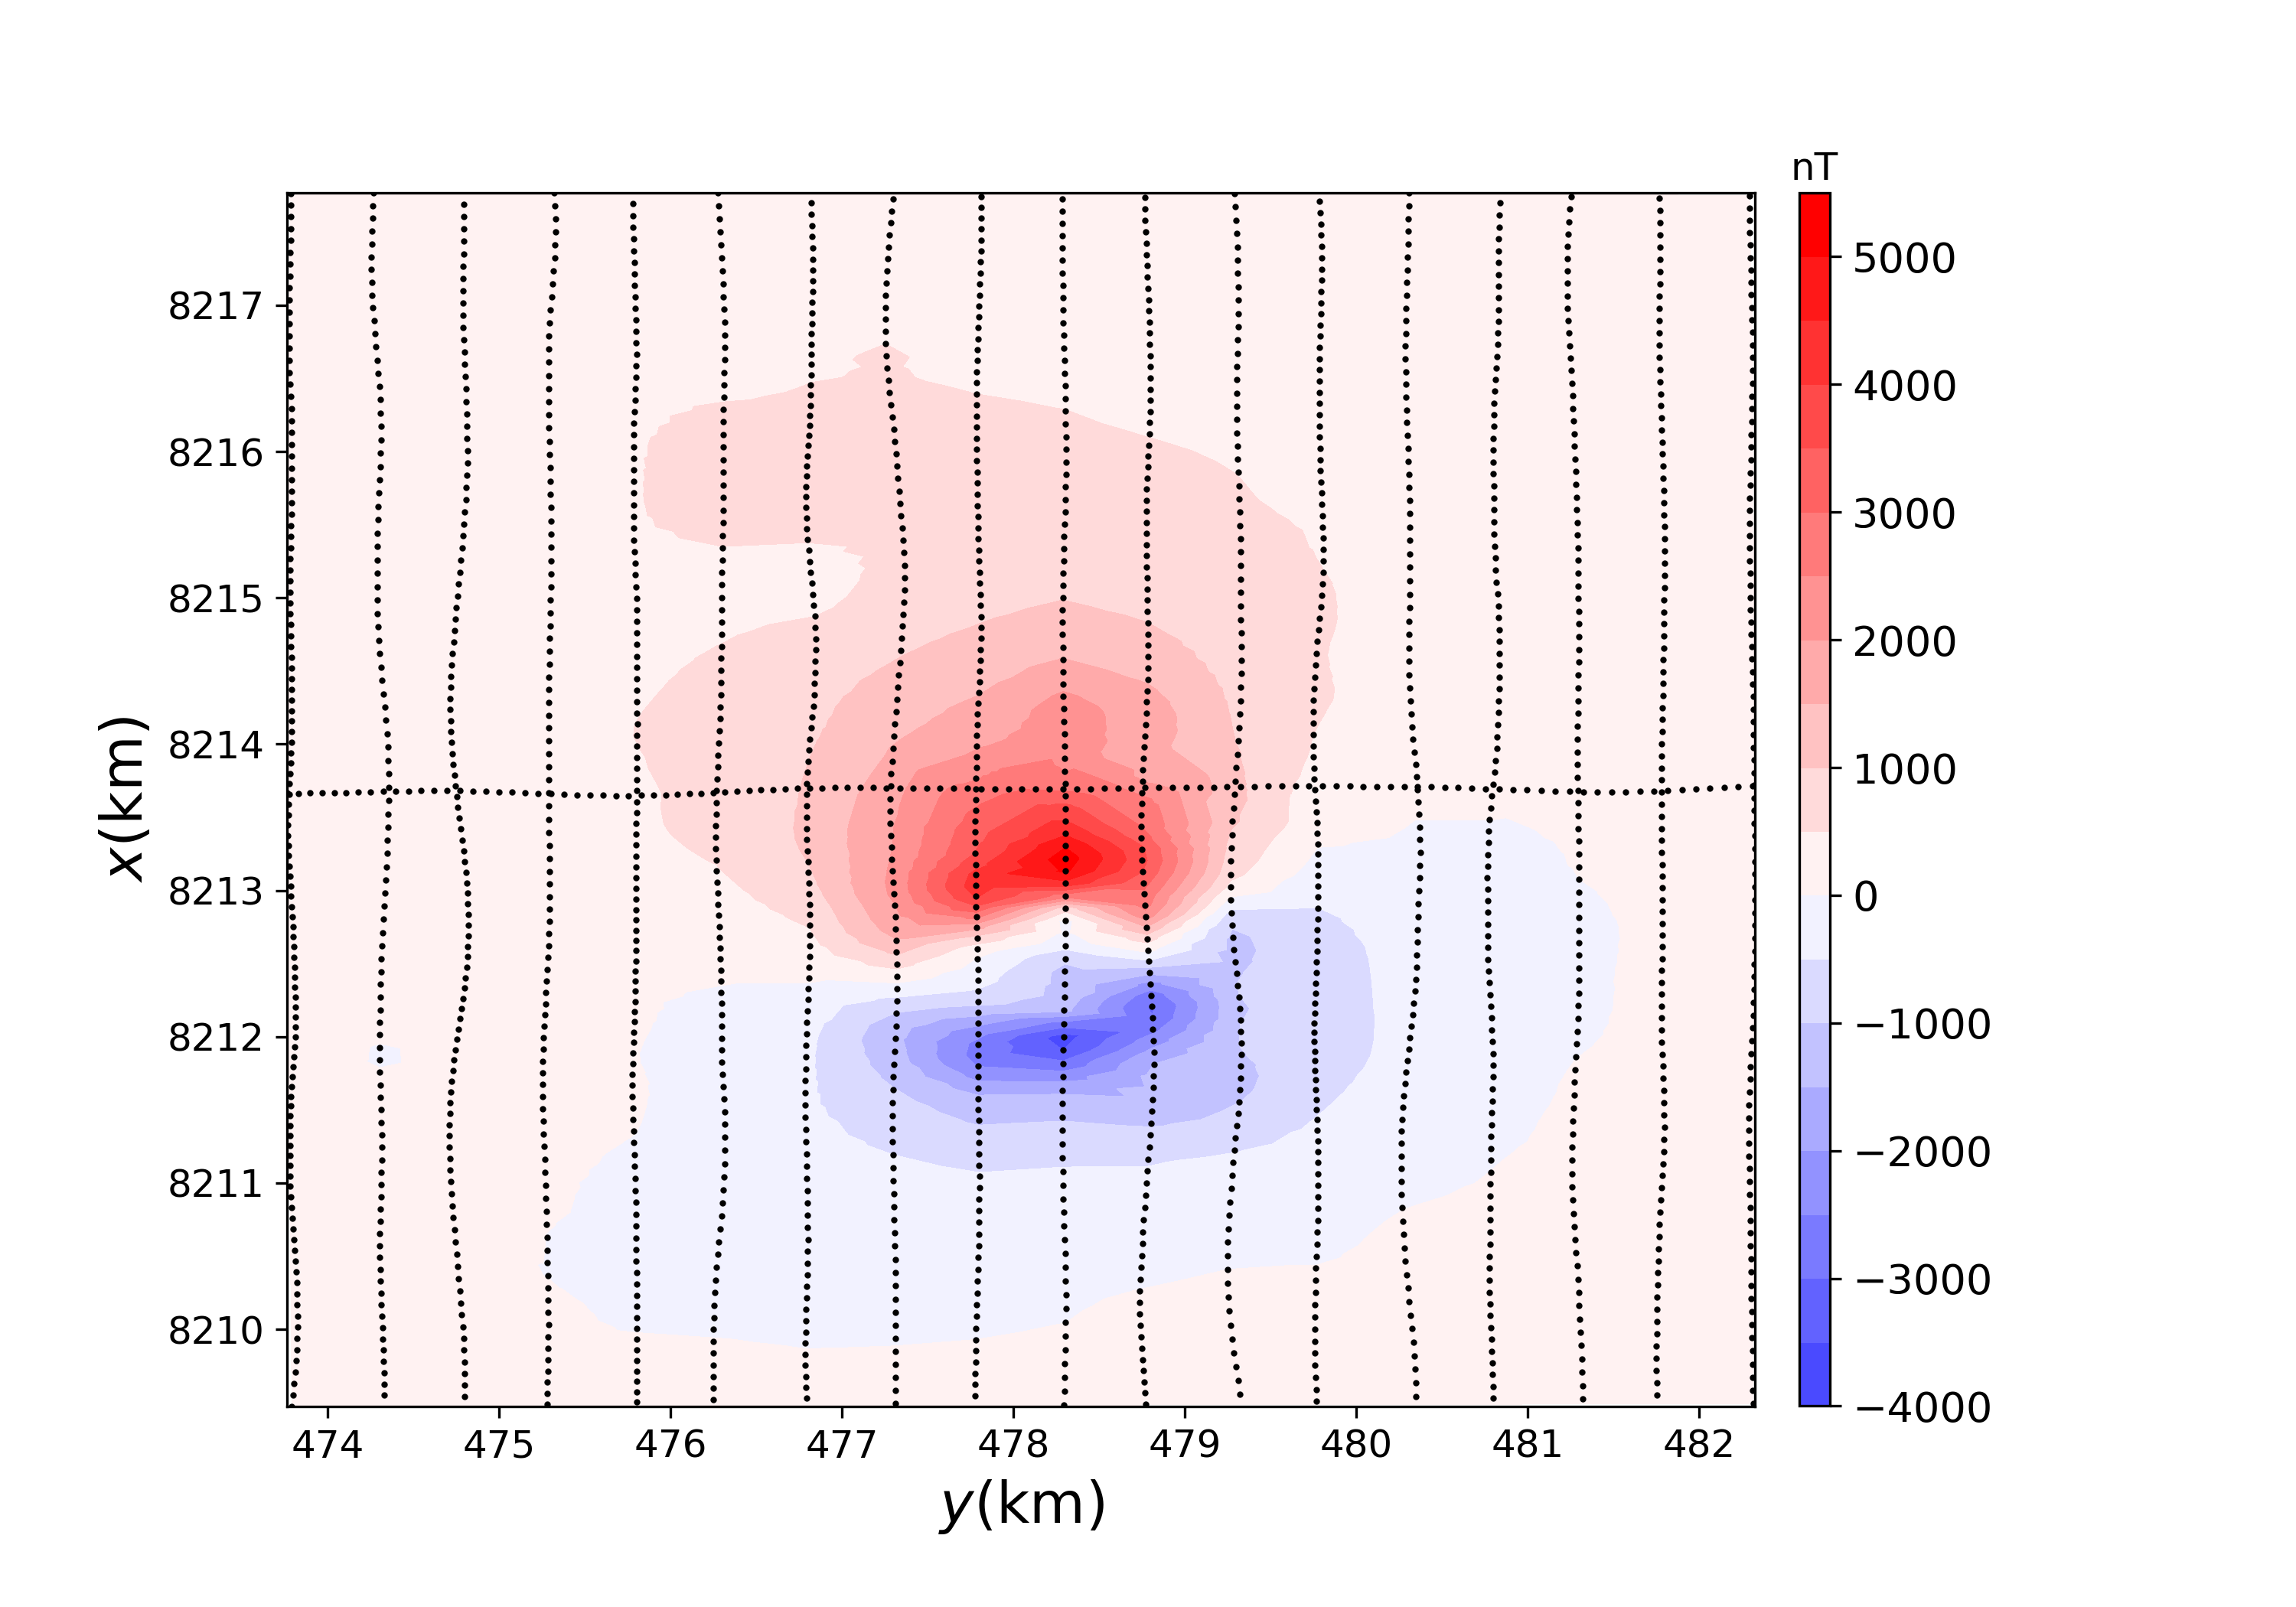
\includegraphics[scale=.5]{figures/diorama_real_data.png}
    \caption{Total-field anomaly of Diorama in GAP. The black dots are the observation points used in this work.
}
    \label{fig:real_data}
\end{figure}

\begin{figure}
    \centering
    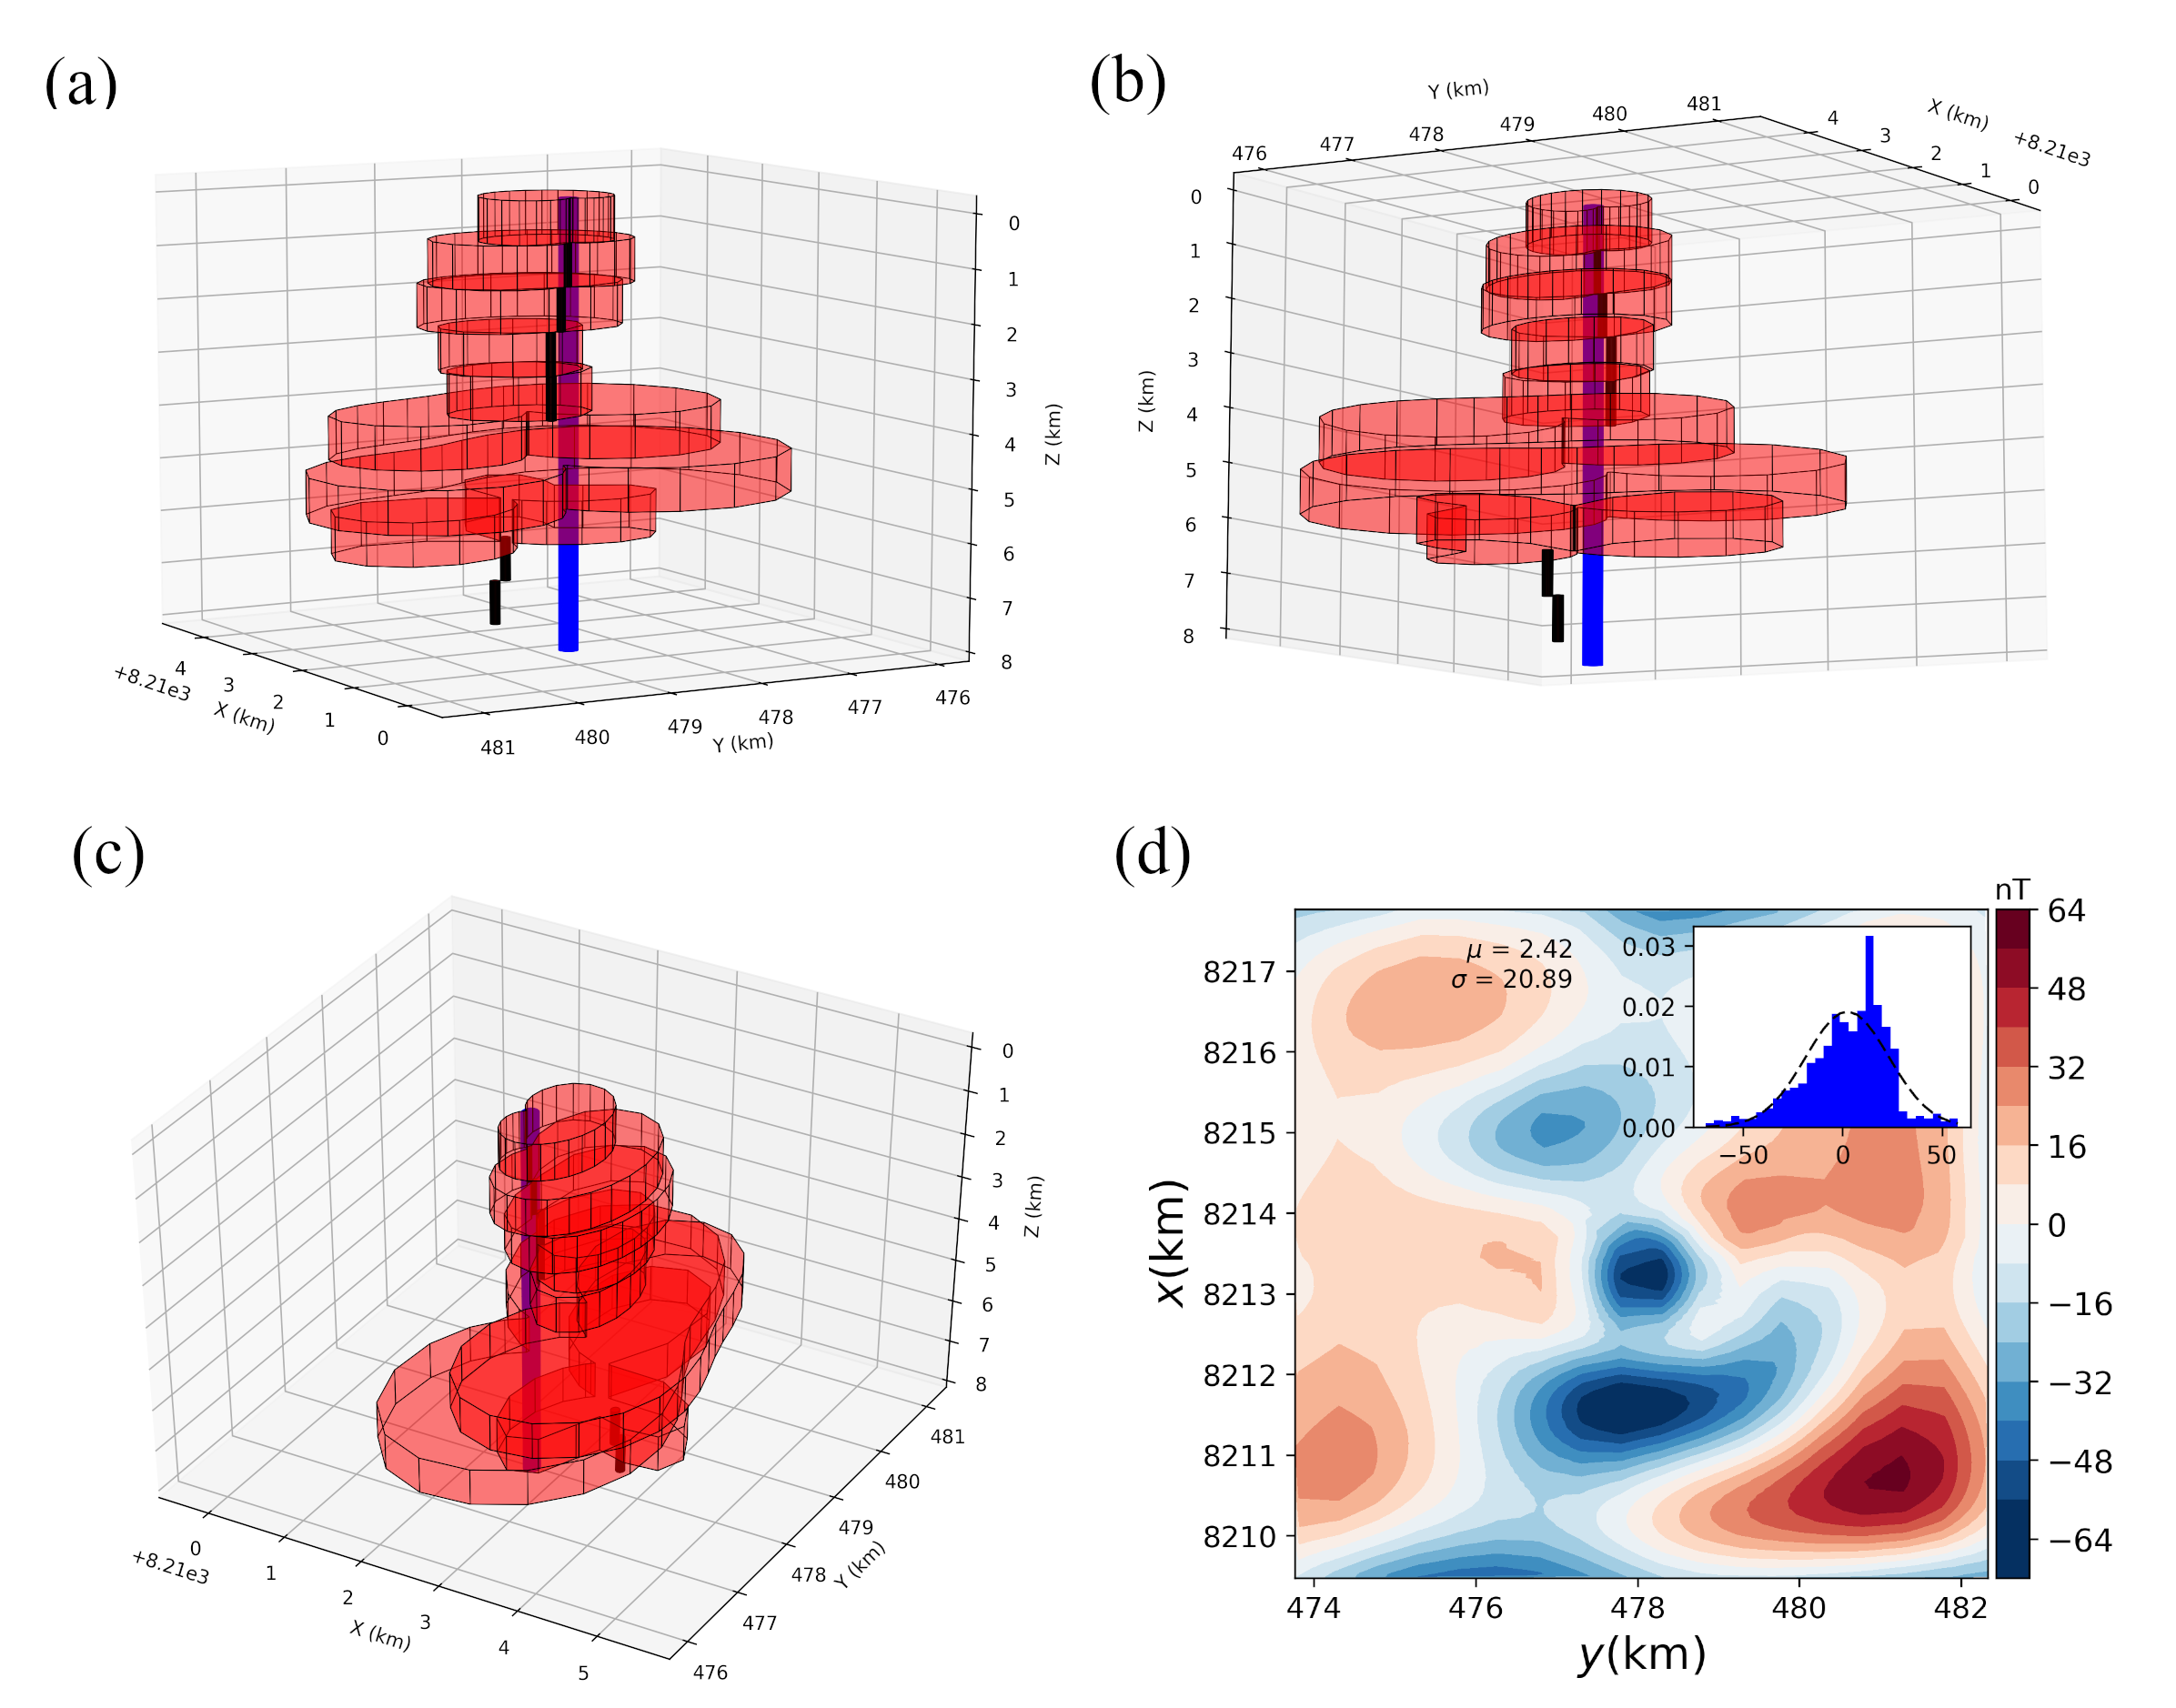
\includegraphics[scale=.75]{figures/real_data_estimates.png}
    \caption{Perspective views of the initial guess (blue cylinder) and the estimated source (red prisms) in (a), (b) and (c). (d) Residuals defined as the difference between the noisy and the predicted (not shown) total-field anomalies and the histogram of the residuals (inset in d) with mean $\mu=2.42$ nT and standard deviation $\sigma=20.89$ nT. The dashed line on the inset is the Gaussian curve for the residuals.
}
    \label{fig:real_result}
\end{figure}